\chapter{Evaluation of raw yield corrections}

To evaluate the ratio between the production yield ratio of the two D-meson species, a number of corrections must be applied to the raw yields. These corrections are necessary to account for the acceptance of the detector, the selection efficiency of \ds and \dpl mesons, the branching ratio of the decay channels, and the feed-down from beauty-hadrons decays. The prompt \ds/\dpl production yield ratio is then obtained by dividing the corrected yield of \ds by the corrected yield of \dpl:
\begin{equation}\label{eq:DsDplusRatio}
        \ds/\dpl = \frac{N_\mathrm{raw}^{\ds}\cdot \fpds}{\aeffpds \cdot \mathrm{BR}^\ds} \cdot \left(\frac{N_\mathrm{raw}^{\dpl}\cdot \fpdpl}{\aeffpdpl \cdot \mathrm{BR}^\dpl}\right)^{-1}\quad ,
\end{equation}
where \aeff is the product of the detector acceptance and the efficiency of D-meson selection, \fp is the fraction of prompt D mesons in the extracted raw yield, and BR is the branching ratio of the considered decay channel. 

In the following sections, a detailed description of the corrections applied to the raw yields is given.

\section{Acceptance and efficiency correction}
The first correction takes into account that of the D mesons produced at midrapidity ($\lvert y\rvert < 0.5$), only a fraction Acc can be detected by the ALICE apparatus, based on the geometry of the detector, and that only a fraction $\varepsilon$ of the detected D mesons passes the selection criteria described in Chapters~\ref{chap:reconstruction} and \ref{chap:RY}.

These corrections are evaluated using a pure sample of \ds and \dpl mesons from Monte Carlo (MC) simulations. To avoid the introduction of biases, a different data sample is used for the evaluation of the acceptance and efficiency corrections than the one used for the ML model training and performance evaluation. Proton-proton collisions are simulated using the \textsc{Pythia~8} event generator~\cite{Bierlich:2022pfr} with colour-reconnection Mode~2~\cite{Christiansen:2015yqa}, and the generated particles are propagated through the ALICE detector using the \textsc{Geant4} transport simulation toolkit~\cite{GEANT4:2002zbu}. Due to the displaced topology of heavy-flavour decays and the continuous readout employed by the ALICE detector, the selection of events with charm or beauty hadrons produces ``fake'' vertices arising from the association of displaced decay tracks, affecting the reconstruction of heavy-flavour hadrons. To overcome this problem, minimum bias events are generated between charm or beauty enriched ones (\emph{gap-triggered} approach). Studies performed using different gap sizes have shown that a gap of 5 minimum bias events between heavy-flavour-injected events reduces the fake-vertex rate to an acceptable level, while keeping the simulation time reasonable.

Special care is taken to ensure that the MC simulation reproduces the experimental conditions and the reconstruction configuration used for data. To improve the description of the spatial resolution in data, a smearing of the track impact parameters is applied via a dedicated workflow (\code{track-tuner}), to reproduce that observed in data. The workflow has been tuned by comparing the impact-parameter resolution in data and MC obtained by fitting their distributions for primary particles. A slightly worse impact-parameter resolution is obtained in data, probably due to residual misalignment of the ITS, as shown in Fig.~\ref{fig:dca_res}, where the impact parameter resolution in the transverse plane and along the beam direction is shown for both data and MC simulations.

\begin{figure}[tbh]
    \begin{center}
    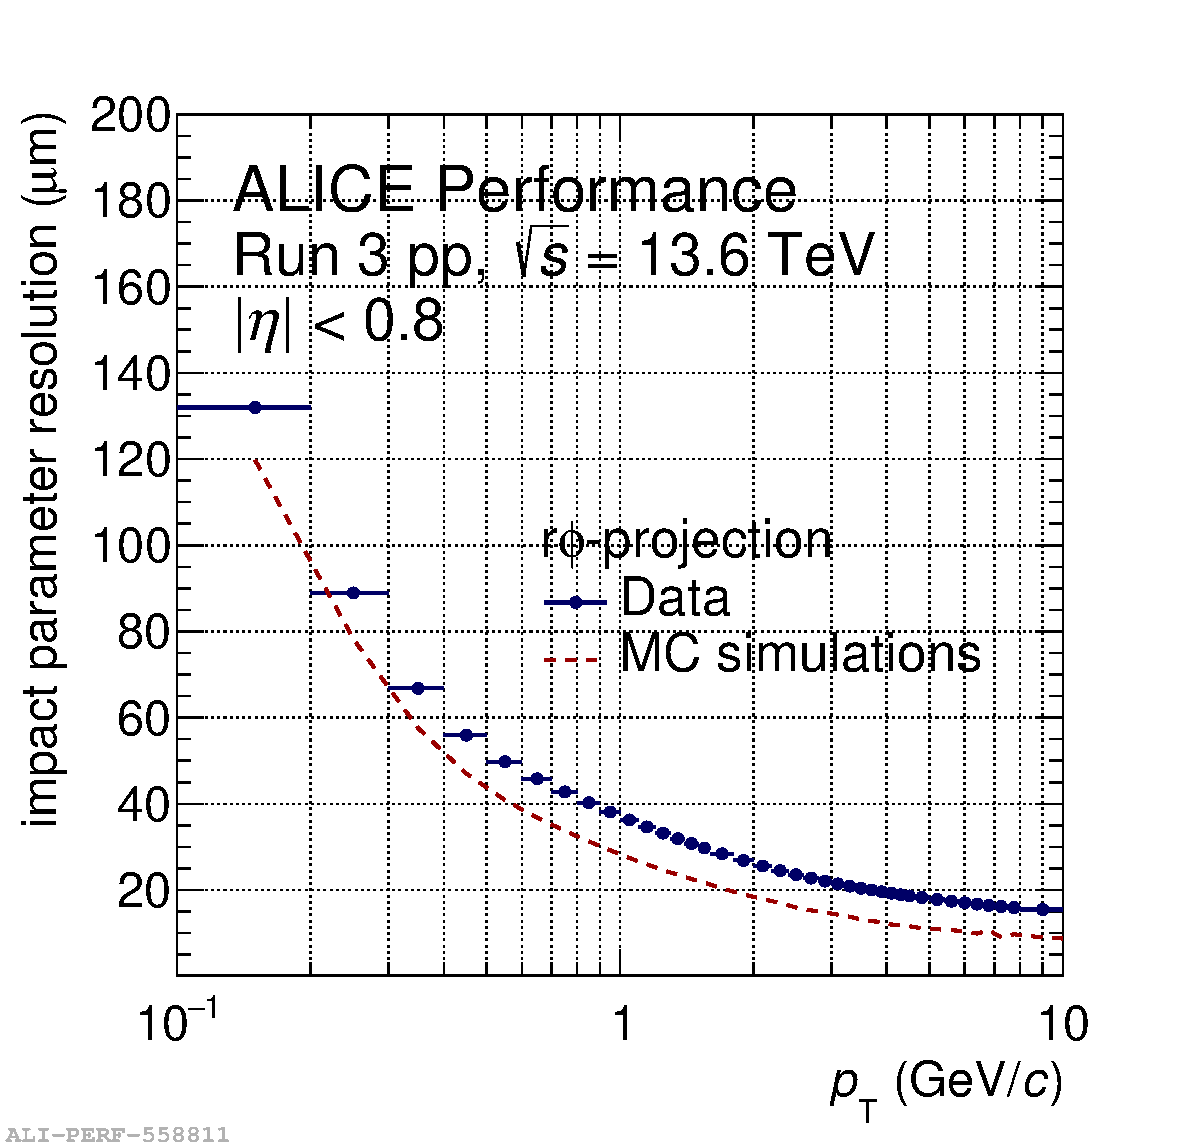
\includegraphics[width=0.48\textwidth]{Figures/Chapter 6/sigmadcaxy_lhc22o_pass4_qm.pdf}
    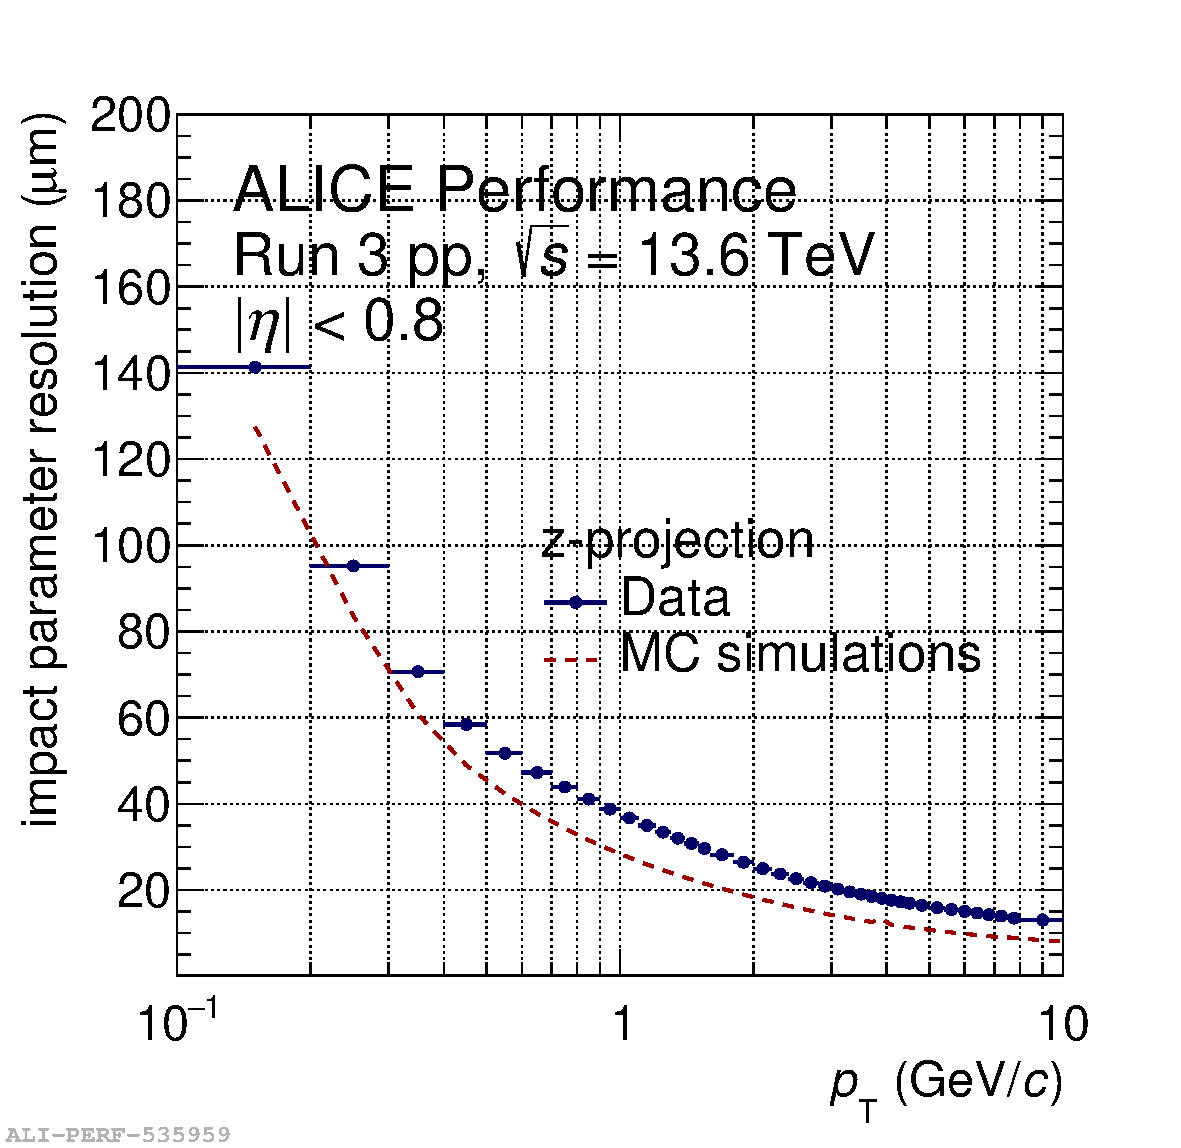
\includegraphics[width=0.48\textwidth]{Figures/Chapter 6/sigmadcaz_lhc22q_pass2_lhcc.pdf}
    \caption{Impact-parameter resolution in the transverse plane (left panel) and beam direction (right panel) of primary particles in data and MC. Figure from ALICE figure repository~\cite{ALICE_figures}.} 
    \label{fig:dca_res} 
    \end{center}
\end{figure}

The \aeff factor is defined as
\begin{equation*}
    \aeff = \frac{N_\mathrm{sel.}^{\lvert y\rvert<0.5}}{N_\mathrm{gen.}^{\lvert y\rvert<0.8}}\quad ,
\end{equation*}
where $N_\mathrm{gen.}^{\lvert y\rvert<0.8}$ is the number of generated D mesons with $\lvert y\rvert<0.8$, and $N_\mathrm{sel.}^{\lvert y\rvert<0.5}$ is the number of D mesons with $\lvert y\rvert<0.5$ that pass the applied selection criteria. The \aeff factor is illustrated in Fig.~\ref{fig:Aeff} for both \ds and \dpl mesons as a function of \pt. Due to the different decay topologies of \ds and \dpl mesons, with the second decaying on average at a larger distance from the primary vertex, the acceptance times efficiency is lower for \ds mesons than for \dpl mesons. For the same reason, the \aeff factor is smaller for promptly-produced D mesons than for non-prompt ones. The correction presents a strong dependence on \pt, with values ranging from about 0.3 at the highest \pt down to about $7\times 10^{-4}$ at the lowest considered \pt interval. The larger Lorentz boost of the D mesons at high \pt results in a more displaced decay vertex, facilitating the identification of \ds and \dpl mesons. In addition, to extract a significant signal at low \pt, where a larger number of background tracks (and therefore combinatorial background candidates) are present, the selection criteria are tightened, reducing the efficiency of the selection.


\begin{figure}[htb]
    \begin{center}
    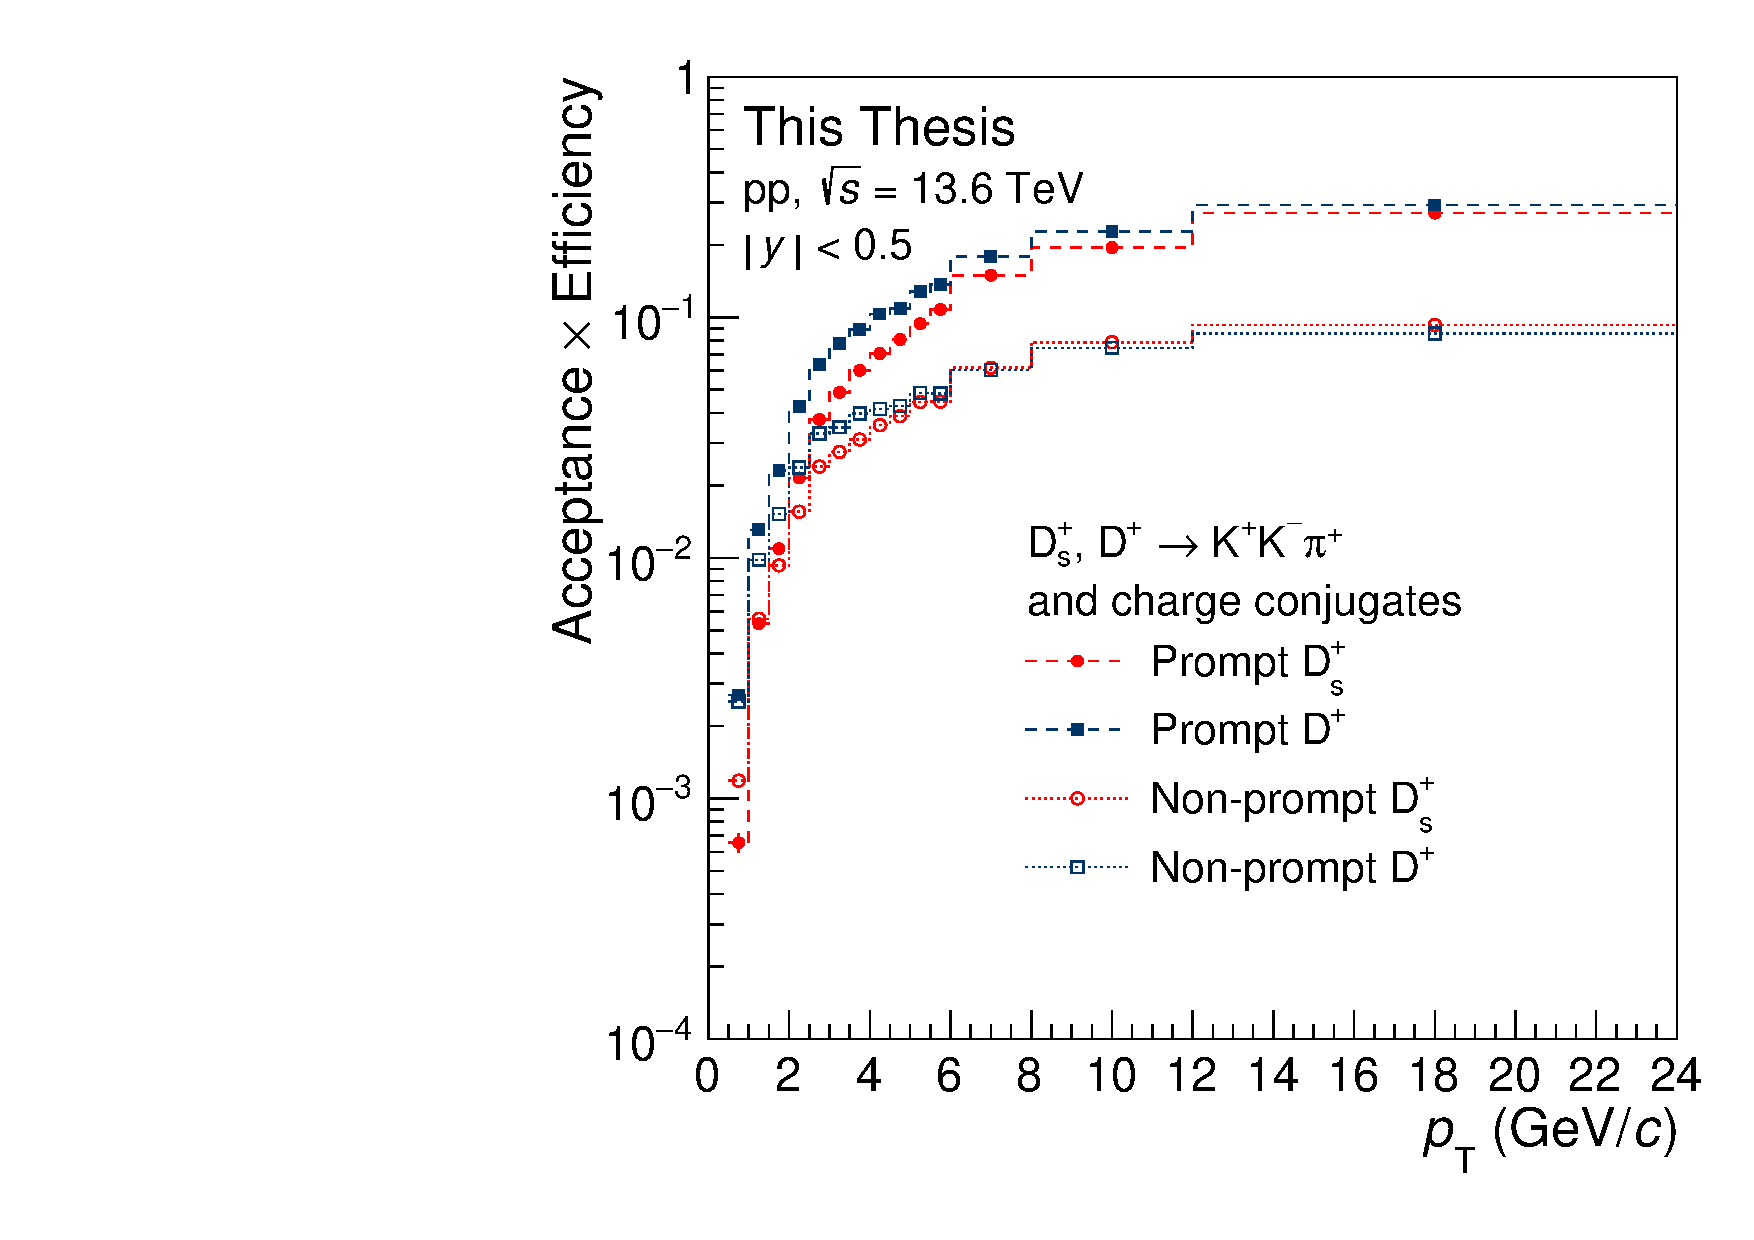
\includegraphics[width=0.7\textwidth]{Figures/Chapter 6/Efficiency_LHC24d3a.pdf}
    \caption{Acceptance-times-efficiency correction factor as a function of \pt for prompt and non-prompt \ds and \dpl mesons.} 
    \label{fig:Aeff} 
    \end{center}
\end{figure}

\section{Prompt fraction correction}
The fraction of prompt \ds and \dpl mesons in the measured raw yield (\fpds and \fpdpl) is estimated with a data-driven method consisting of varying the BDT probability threshold used for the candidate selection. This variation changes the balance between prompt and non-prompt signals and exploits their different trend with the BDT output score to disentangle their contributions to the raw yield. Introduced in Run~2 in Ref~\cite{ALICE:2021mgk}, this approach exploits the relationship between the raw yield and the number of produced prompt and non-prompt D mesons:
\begin{equation}\label{eq:fp_rawyields}
    N_\mathrm{raw} = N_\mathrm{prompt}\times\aeffp + N_\mathrm{non\text{-}prompt} \times \aeffnp\quad .
\end{equation}
\vspace{0.1cm}
Eq.~\ref{eq:fp_rawyields} holds for every chosen BDT selection criterion, which defines the \aeffp and \aeffnp correction factors. As the \aeff factors can be determined from MC simulations as described in the previous section, Eq.~\ref{eq:fp_rawyields} contains only two unknown variables, $N_\mathrm{prompt}$ and $N_\mathrm{non\text{-}prompt}$. They can be found by changing the BDT working point and extracting the corresponding raw yield. However, a single variation of the selection criteria may lead to large uncertainties, as a small change in the \aeff correction does not add a lot of information. To overcome this issue, the BDT threshold values are varied several times to span a wide range of \aeffp and significantly change the \fp in the raw yield. For each selection criterion i, the acceptance-times-efficiency factor is calculated for prompt $\aeffp^\mathrm{i}$ and non-prompt $\aeffnp^\mathrm{i}$ D mesons, and the raw yields $N_\mathrm{raw}^\mathrm{i}$ are extracted by fitting the invariant mass distribution of candidates passing the selections. By including the whole set of selection criteria, a system of equations can be defined:
\begin{equation*}
    \begin{cases}
        N_\mathrm{raw}^1 = N_\mathrm{prompt}\times\aeffp^1 + N_\mathrm{non\text{-}prompt} \times \aeffnp^1\\
        N_\mathrm{raw}^2 = N_\mathrm{prompt}\times\aeffp^2 + N_\mathrm{non\text{-}prompt} \times \aeffnp^2\\
        \vdots\\
        N_\mathrm{raw}^\mathrm{n} = N_\mathrm{prompt}\times\aeffp^\mathrm{n} + N_\mathrm{non\text{-}prompt} \times \aeffnp^\mathrm{n}
    \end{cases}
    \quad ,
\end{equation*}
For $\mathrm{n>2}$, the system of equations is overconstrained, and the solution can be found through a minimisation procedure. The system of equations can be written in matrix notation as
\begin{equation*}
    \begin{pmatrix}
        \aeffp^1 & \aeffnp^1\\
        \aeffp^2 & \aeffnp^2\\
        \vdots & \vdots\\
        \aeffp^\mathrm{n} & \aeffnp^\mathrm{n}
    \end{pmatrix}
    \begin{pmatrix}
        N_\mathrm{prompt}\\
        N_\mathrm{non\text{-}prompt}
    \end{pmatrix}
    -
    \begin{pmatrix}
        N_\mathrm{raw}^1\\
        N_\mathrm{raw}^2\\
        \vdots\\
        N_\mathrm{raw}^\mathrm{n}
    \end{pmatrix}
    =
    \begin{pmatrix}
        \delta^1\\
        \delta^2\\
        \vdots\\
        \delta^\mathrm{n}
    \end{pmatrix}
    \quad ,
\end{equation*}
where $\delta^\mathrm{i}$ are the residuals arising from the inexact solution of the i-th equation in the system due to the uncertainty on the raw yield and \aeff correction factors. For each selection criterion, the uncertainty on $\delta^\mathrm{i}$ is estimated by propagating the uncertainties on the raw yield and \aeff factors as
\begin{equation*}
    \sigma_\mathrm{i}^2 = \sigma_{N_\mathrm{raw}^\mathrm{i}}^2 + N_\mathrm{prompt}\times\sigma^2_{\aeffp^\mathrm{i}} + N_\mathrm{non\text{-}prompt}\times\sigma^2_{\aeffnp^\mathrm{i}}\quad .
\end{equation*}
Given that the corrected yields are unknown variables, an iterative procedure was used to define the total uncertainty: in the first step 
$N_{\mathrm{prompt}}$ and $N_{\mathrm{non\text{-}prompt}}$ are set to zero and only the uncertainty on the raw yields is taken into account. From the second iteration the corrected yields $N_{\mathrm{prompt}}$ and $N_{\mathrm{non\text{-}prompt}}$ obtained in the previous step are also used. This iteration is repeated until the difference between the corrected yields evaluated in two subsequent iterations falls below a predefined threshold.

The solution of the system of equations is found by minimising the residuals with a least-squares method, where the $\chi^2$ is defined as 
\begin{equation*}
    \chi^2 = \pmb{\delta}^\mathrm{T}\mathbf{C}^{-1}\pmb{\delta}\quad ,
\end{equation*}
where $\pmb{\delta}$ is the vector of residuals and $\mathbf{C}$ is the covariance matrix of the residuals.

In this analysis, the BDT threshold is fixed for the background score, at a tighter value than the one used to extract the central raw yields to ensure the convergence of the invariant mass fits. The minimum probability for being a non-prompt D meson is varied in different ranges for the two hadrons, to guarantee that a large enough variation in the \fnp is achieved. Because the selection criterion is increasingly tightened, the $\mathrm{i+1}$-th selected sample will be entirely contained in the $\mathrm{i}$-th one. The residuals $\delta^\mathrm{i}$ will therefore exhibit a degree of correlation. The off-diagonal elements $\sigma_\mathrm{i,j}$ of the covariance matrix $\mathbf{C}$, which are the covariance between the residuals of the i-th and j-th selection criteria, can be estimated as 
\begin{equation*}
    \sigma_\mathrm{i,j} = \rho_\mathrm{i,j}\sigma_\mathrm{i}\sigma_\mathrm{j}\quad ,
\end{equation*}
where it can be demonstrated~\cite{cowan1998statistical} that the correlation coefficient $\rho_\mathrm{i,j}$ is given by 
\begin{equation*}
    \rho_\mathrm{i,j} = \frac{\sigma_\mathrm{i}}{\sigma_\mathrm{j}}\quad 
\end{equation*}
if the measurement i uses the same data as the measurement j. 
\begin{sloppypar}
The minimisation procedure described above leads to the determination of $N_\mathrm{prompt}$ and $N_\mathrm{non\text{-}prompt}$, which are independent of the applied selection criteria.

The results for the evaluation of the \ds \fp correction factor in the $1.5<\pt<2.0$~\gevc interval is shown in Fig.~\ref{fig:fp}. In the top-left panel, the correlation factor $\rho$ is shown for the different selection criteria; in the top-right panel, the \aeff factors are shown as a function of the BDT selection criterion for both prompt and non-prompt \ds mesons; in the bottom-left panel, the relative contribution of the prompt and non-prompt component to the extracted \ds raw yields is shown as a function of the ML selections. Finally, in the bottom-right panel, the extracted yields are fitted using a template fit, using the \aeffpds and \aeffnpds evolution as a function of the BDT selection criterion as input. The minimisation procedure described above can in fact be interpreted as a template fit to the extracted raw yieds, where the templates are the \aeff factors. The prompt and non-prompt components, obtained for each BDT-based selection from the minimisation procedure as $\aeffp\times N_\mathrm{prompt}$ and $\aeffnp\times N_\mathrm{non\text{-}prompt}$ are represented with red and blue filled histograms, respectively. Their sum is reported by the green histograms. Given the small $\chi^2$/ndf value obtained from the fit, the \fp factor is considered to be well determined. The leftmost data point of each distribution corresponds to the looser selection on the BDT non-prompt score, while the rightmost one corresponds to the strictest selection, which is expected to preferentially select non-prompt D mesons. 

\begin{figure}[htb]
    \begin{center}
    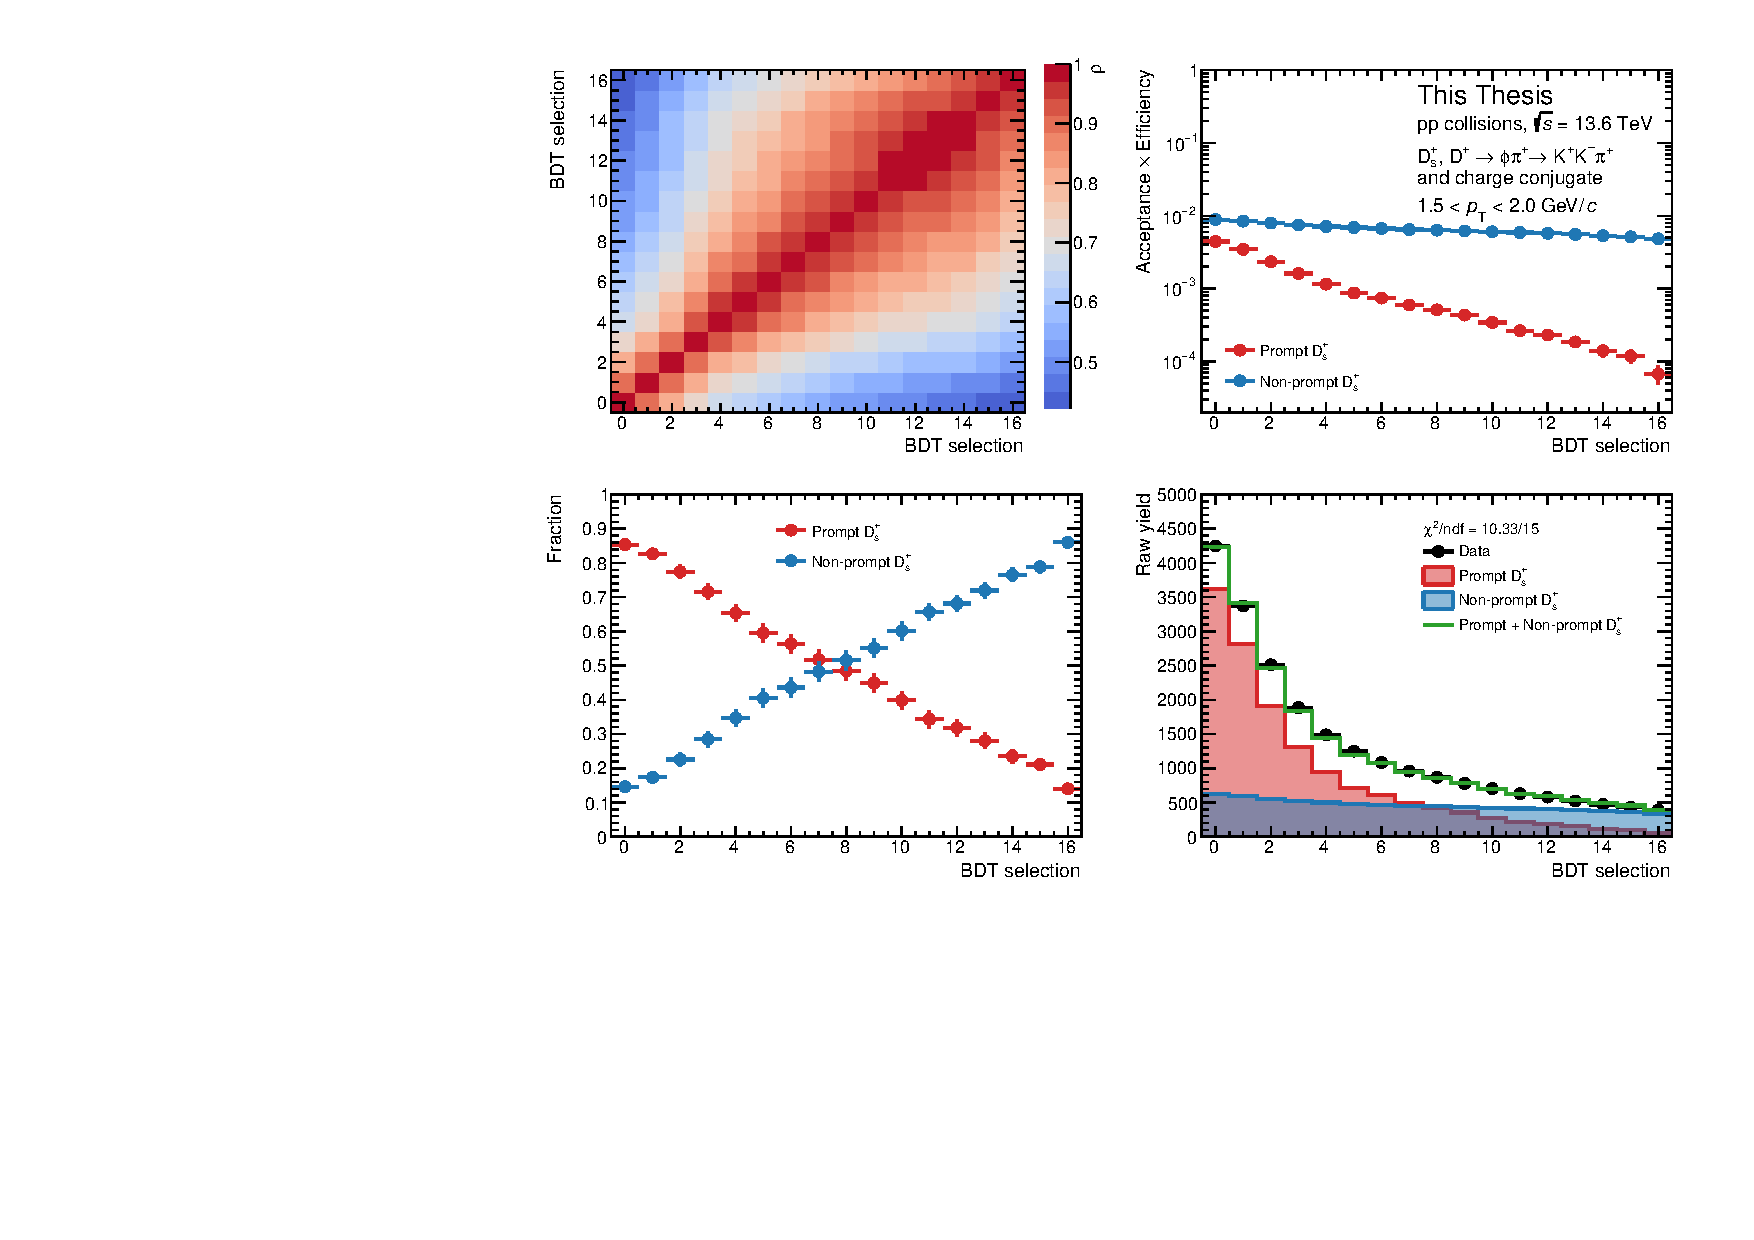
\includegraphics[width=\textwidth]{Figures/Chapter 6/DsPromptFrac.pdf}
    \caption{Results for the evaluation of the \ds \fp correction factor in the $1.5<\pt<2.0$~\gevc interval. The correlation factor $\rho$ (top-left panel), \aeff factors for both prompt and non-prompt \ds mesons (top-right panel), prompt and non-prompt fraction in the extracted \ds raw yields (bottom-left panel) and contribution of prompt and non-prompt to the extracted raw yields (bottom-right panel) are shown as a function of the BDT selection criterion.} 
    \label{fig:fp} 
    \end{center}
\end{figure}

The \fp factor is then calculated, for each D-meson species and for any given selection criterion with efficiencies \aeffp and \aeffnp for prompt and non-prompt D mesons respectively, as
\end{sloppypar}
\begin{equation*}
    \fp = \frac{N_\mathrm{prompt}\times\aeffp}{N_\mathrm{prompt}\times\aeffp + N_\mathrm{non\text{-}prompt}\times\aeffnp}\quad .
\end{equation*}

As a cross-check, the \fp factor is also estimated using a theory-driven approach~\cite{ALICE:2017olh}, which relies on FONLL~\cite{Cacciari:1998it} prediction for beauty-hadron production and the decay kinematic description of \textsc{Pythia~8}~\cite{Bierlich:2022pfr} for estimating the \pt differential cross section of non-prompt D mesons. The \fp factor is then calculated for each D-meson species as 
\begin{equation*}
    \fp = 1-\left.\frac{\de^2\sigma}{\de\pt\de y}\right\vert_\mathrm{FONLL+\textsc{Pythia}~8}^\mathrm{non\text{-}prompt}\times\frac{\aeffnp \Delta y \Delta\pt \mathrm{BR} \mathcal{L}_\mathrm{int}}{\frac{1}{2}\times N_\mathrm{raw} }\quad ,
\end{equation*}
where $\Delta y$ and $\Delta\pt$ are the rapidity and \pt intervals, respectively, $\mathcal{L}_\mathrm{int}$ is the integrated luminosity, corresponding to \SI{1}{\per\pico\barn}, $N_\mathrm{raw}$ is the raw yield of the considered D meson, and the factor 1/2 takes into account that both particle and antiparticles are selected. 

A comparison between the \fp correction factors for \ds and \dpl mesons obtained with the two methods is illustrated in Fig.~\ref{fig:fp_comparison}. A good level of agreement is observed between the two results. For the evaluation of the central \fp values, the data-driven method is used, as it is not sensitive to possible shortcomings in the theoretical description of $\mathrm{b\overline{b}}$ production which may affect the theory-driven approach.

\begin{figure}
    \begin{center}
    \includegraphics[width=0.48\textwidth]{example-image-a}
    \includegraphics[width=0.48\textwidth]{example-image-b}
    \caption{\fp correction factor for \ds (left) and \dpl (right) mesons as a function of \pt. The results obtained with the data-driven method are compared with those exploiting a theory-driven approach.} 
    \label{fig:fp_comparison} 
    \end{center}
\end{figure}

\section{Branching ratio correction}
\begin{sloppypar}

The branching ratio correction is applied to account for the fact that of the produced \ds and \dpl mesons, only those decaying into a KK$\pi$ final state are reconstructed. The values of the branching ratios for the considered decays are taken from Ref.~\cite{pdg}, and correspond to \mbox{$\mathrm{BR}(\ds) = (2.21\pm0.06)\times10^{-2}$} and \mbox{$\mathrm{BR}(\dpl) = \left((2.69^{+0.07}_{-0.08})\times10^{-3}\right)$}. Since these values are not evaluated through the analysis carried out in this Thesis, but rather taken from a global fit reported in a different publication, a systematic uncertainty is assigned to account for the uncertainty provided by the PDG. The uncertainty is propagated to the \ds/\dpl production yield ratio with a gaussian approach, yielding an asymmetric $^{+3.7}_{-4.0}\%$ uncertainty on the ratio.
\end{sloppypar}

\section{Systematic uncertainties}
Measurements of particle production yield ratios allow for the cancellation of some related systematic uncertainties, such as that related to luminosity. In addition, the reconstruction of \ds and \dpl mesons through the same decay channel allows for the cancellation of supplementary sources of systematic uncertainties, such as those related to tracking and PID efficiency, thereby enhancing the precision of the results. However, the measurement is still affected by several sources of systematic uncertainties, due to arbitrary choices made in the analysis, or the need to rely on MC simulations, which could not perfectly reproduce the data. 

\subsection{BDT selection efficiency}
The choice of the set of BDT threshold values used to extract the raw yields, albeit being driven by a defined criterion through the maximisation of the significance on a subsample of the data, remains an arbitrary choice. Variations in the ML selection criteria may lead to variations in the extracted raw yields, and therefore in the \ds/\dpl production yield ratio. The systematic uncertainty on the BDT selection efficiency is estimated by varying the BDT threshold values on prompt and background probabilities, independently and then simultaneously, for a total of \textcolor{red}{XX} variations. To avoid extreme variations of the selection criteria, the \aeffp for both D-meson species is required to be within 30\% of that for the central selections. To 


The uncertainty is estimated by taking the difference between the \fp factors obtained with the varied and nominal BDT threshold values, and is found to be about 1\% for both D-meson species.



\textcolor{red}{aggiungere pt shape (perchè non lo aggiungiamo (abbiamo anche fatto un check))}